\documentclass{amsbook}
\usepackage{../HBSuerDemir}

\title{b2p1-124}
\author{Murat Buldu}

\begin{document}
\hPage{b2p1/124}
\par
    \underline{Projections of vectors}:
\par
    Let \(\hVec{OP}\) be a vector and \(Ot\) be an axis with a unit vector \(\hVec{e}\) along it. If \(P^{\prime}\) is the projection of \(P\) on \(Ot\) (which is the intersections of \(Ot\) with the plane through \(P\) perpendicular to \(Ot\)), then \(\hVec{OP^{\prime}}\) is the \underline{vector projection} (\underline{Vector compoment}),and the coordinate of \(P^{\prime}\) is the \underline{scalar projections} (\underline{scalar compoment}) of \(\hVec{OP}\) on \(Ot\). (See Fig.)

\begin{minipage}{0.5\textwidth}
\par
Now consider a second vector \(\hVec{OQ}\) and the vector \(\hVec{OR} = \hVec{OP} + \hVec{OQ}\) where \(\hVec{OQ} = \hVec{PR}\). Then the projection of \(\hVec{OR}\) on \(Ot\) is 
\(\hVec{OR^{\prime}} = \hVec{OP^{\prime}} + \hVec{P^{\prime}R^{\prime}}\) which is the sum of projections(compoments).

\end{minipage}
\begin{minipage}{0.5\textwidth}
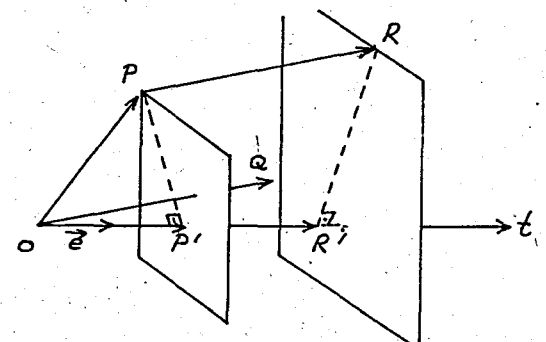
\includegraphics[width=0.96\textwidth]{b2p1-124-fig01.png}
\end{minipage}
\par
    Obviously the scalar component of the sum \(\hVec{OR}\) is the sum of scalar components of \(\hVec{OP}\), \(\hVec{OQ}\).
\par
    Now, taking coordinate axes \(Ox, Oy, Oz\) instead of \(Ot\) with respective unit vectors
    \[i = (1,0,0), j = (0,1,0), k = (0,0,1) \]
    along positive parts and denoting the projections of \(P(x,y,z)\) on the axes and \(xy-plane\) by \(X,Y,Z\) and \(P^{\prime}\) we have
\par
\begin{minipage}{0.5\textwidth}
    \begin{align*} 
        \hVec{OP} &= \hVec{OP^{\prime}} + \hVec{P^{\prime}P} \\ 
                &= \hVec{OX} + \hVec{OY} + \hVec{OZ}
    \end{align*}
        since \(\hVec{OX} + \hVec{OY} = \hVec{OP^{\prime}}\) and \(\hVec{OZ} = \hVec{P^{\prime}P}\)
    \par
        Then
        \[\hVec{OP^{\prime}} = xi + yj + zk\]
        where \(xi\), \(yj\), \(zk\) are vector
\end{minipage}
\begin{minipage}{0.5\textwidth}
    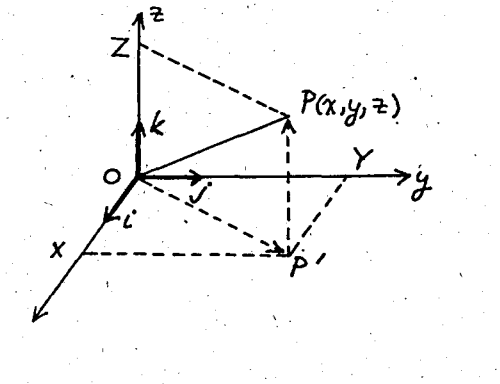
\includegraphics[width=0.96\textwidth]{b2p1-124-fig02.png}
\end{minipage}

\end{document}